\subsection{Трекинг}

После получения результатов модели детектирования было необходимо рассмотреть несколько алгоритмов последующего трекинга, такие как OC-SORT, ByteTrack, DeepSORT и StrongSORT.

Лучшим показавшим себя алгоритмом трекинга для данной задачи по результатам экспериментов стал StrongSORT, который наиболее точно работал с часто пропадающими из кадра и пересекающими траектории друг друга объектами, показав наивысшую из полученных точностей, поскольку одним из главных его преимуществ является способность работать с полными и частичными окклюзиями.

Для данного алгоритма была реализована модификация его официальной версии с целью интеграции с YOLOv5, после чего был проведен запуск трекинга на основе полученной ранее модели детектирования. Пример достигнутого результата приведен на Рис. \ref{img:11-1}, на котором для каждого объекта указаны его класс и уникальный номер.

\vspace{0.5cm}

\begin{figure}[ht]
    \centering
    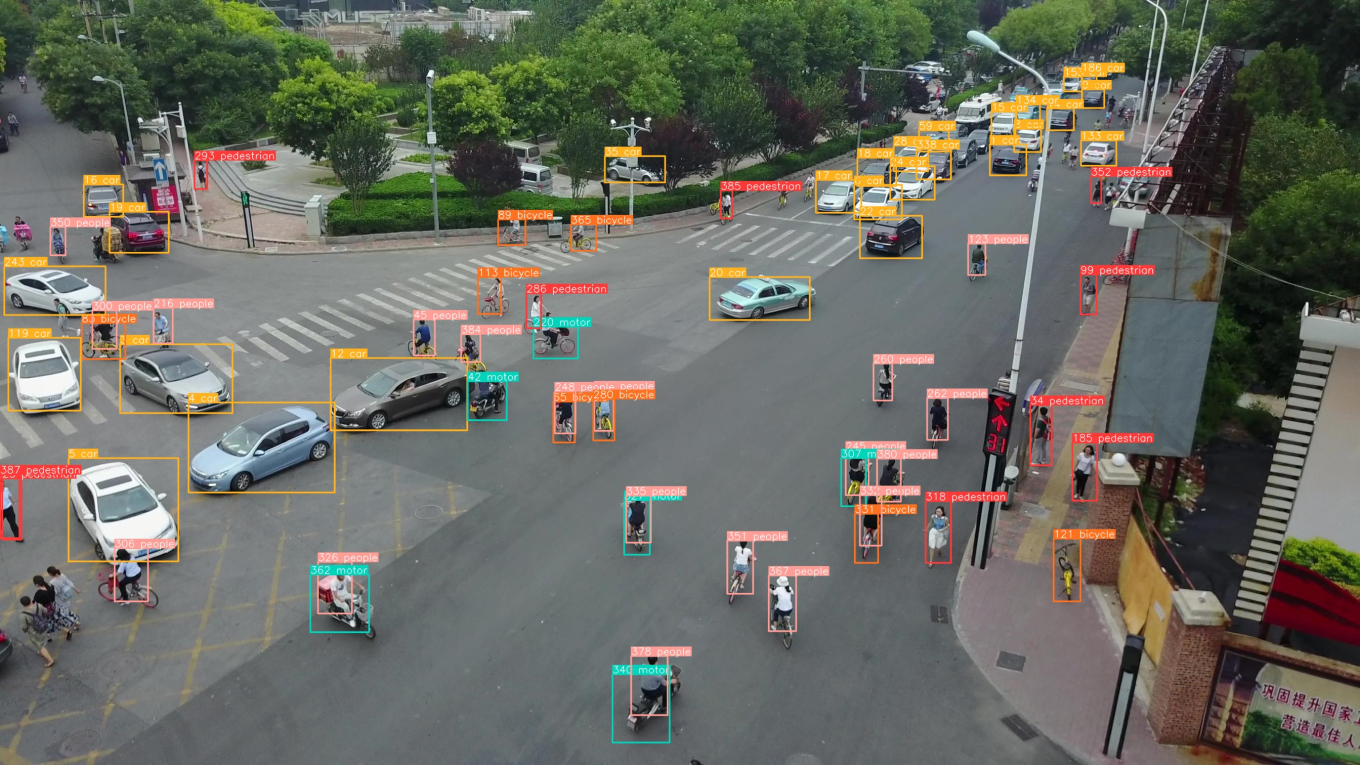
\includegraphics[width=0.85\textwidth]{11-1}
    \caption{Пример кадра из видео, к которому применен алгоритм трекинга StrongSORT}
    \label{img:11-1}
\end{figure}

Однако классический StrongSORT содержит в себе проблемы в построении плавных траекторий объектов по причине наличия нестабильного движения камер с беспилотных летательных аппаратов, вследствие чего некоторые объекты между кадрами теряются, а ограничивающие рамки имеют характер дрожания.

Для решения указанной проблемы в модификацию StrongSORT были добавлены линейная интерполяция и гауссовское сглаживание (GSI), описанные ранее в работе. После применения к трекингу данной постобработки без подбора параметров были получены траектории объектов, нестабильные при резких поворотах и подъемах камер, что наблюдается на Рис. \ref{img:11-2}, где ограничивающие рамки объектов после изменения положения камеры сильно сместились относительно реальных положений объектов.

\vspace{0.5cm}

\begin{figure}[ht]
    \centering
    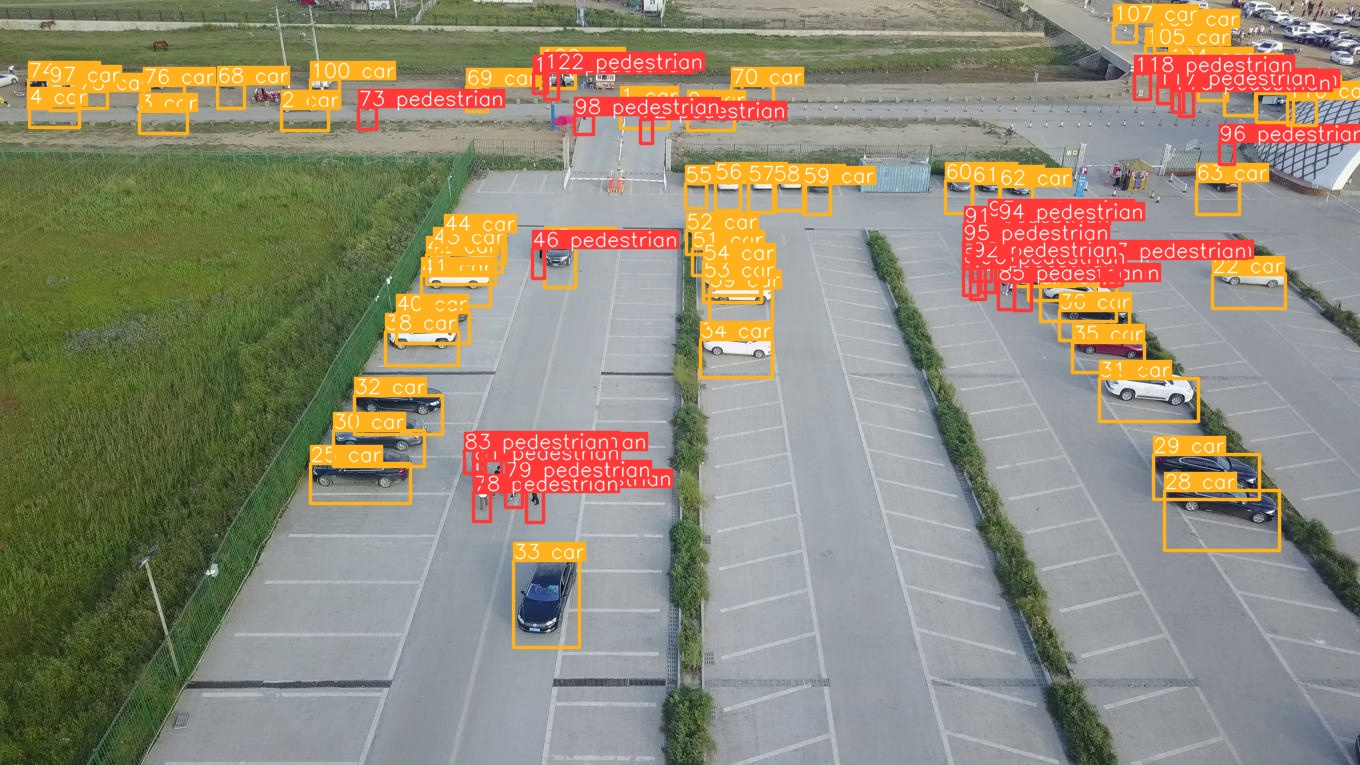
\includegraphics[width=0.85\textwidth]{11-2}
    \caption{Пример ошибок в трекинге по причине движения камеры}
    \label{img:11-2}
\end{figure}

В данном алгоритме постобработки имеется 2 управляющих параметра: $interval$ и $\tau$, первый из которых отвечает за количество кадров, участвующих в поиске объекта, а второй -- за степень сглаживания траектории. В результате экспериментов с их варьированием были получены оптимальные для данной задачи значения:

\begin{equation}
    interval = 5,
\end{equation}

\begin{equation}
    \tau = 9.
\end{equation}

В результате применения полученных значений параметров значительно уменьшилось влияние движения камеры на полученные траектории.
